\begin{exerciseS}[Sorgente lineare nel piano]
 Utilizzando l'espressione dela velocità indotta da una sorgente puntiforme di intensità unitaria,
\begin{equation}
 \bm{u} = \dfrac{1}{2\pi r} \bm{\hat{r}} \ ,
\end{equation}
 dimostrare che la velocità indotta nel punto $\bm{P}$ da una sorgente di intensità unitaria uniforme distribuita sul segmento che congiunge i due punti $\bm{N}_1$, $\bm{N}_2$ vale
\begin{equation}
 \bm{u} = - \dfrac{1}{2\pi} \ln \dfrac{|\bm{r}_2|}{|\bm{r}_1|} \bm{\hat{x}} 
 + \dfrac{1}{2\pi} \beta \bm{\hat{y}} \ ,
\end{equation}
 essendo $\bm{\hat{x}}$, $\bm{\hat{y}}$ i versori in direzione tangente e normale al segmento $\bm{N}_1 \bm{N}_2$, i vettori $\bm{r}_i = \bm{P} - \bm{N}_i$, $i = 1:2$ e $\beta$ l'angolo compreso tra il vettore $\bm{r}_1$ e il vettore $\bm{r}_2$, positivo se si deve ruotare il vettore $\bm{r}_1$ in senso antiorario per farlo coincidere con $\bm{r}_2$.
\end{exerciseS}

\begin{center}
\begin{figure}[h]
\centering
\includegraphics[width=0.40\textwidth]{./fig/pointSource}
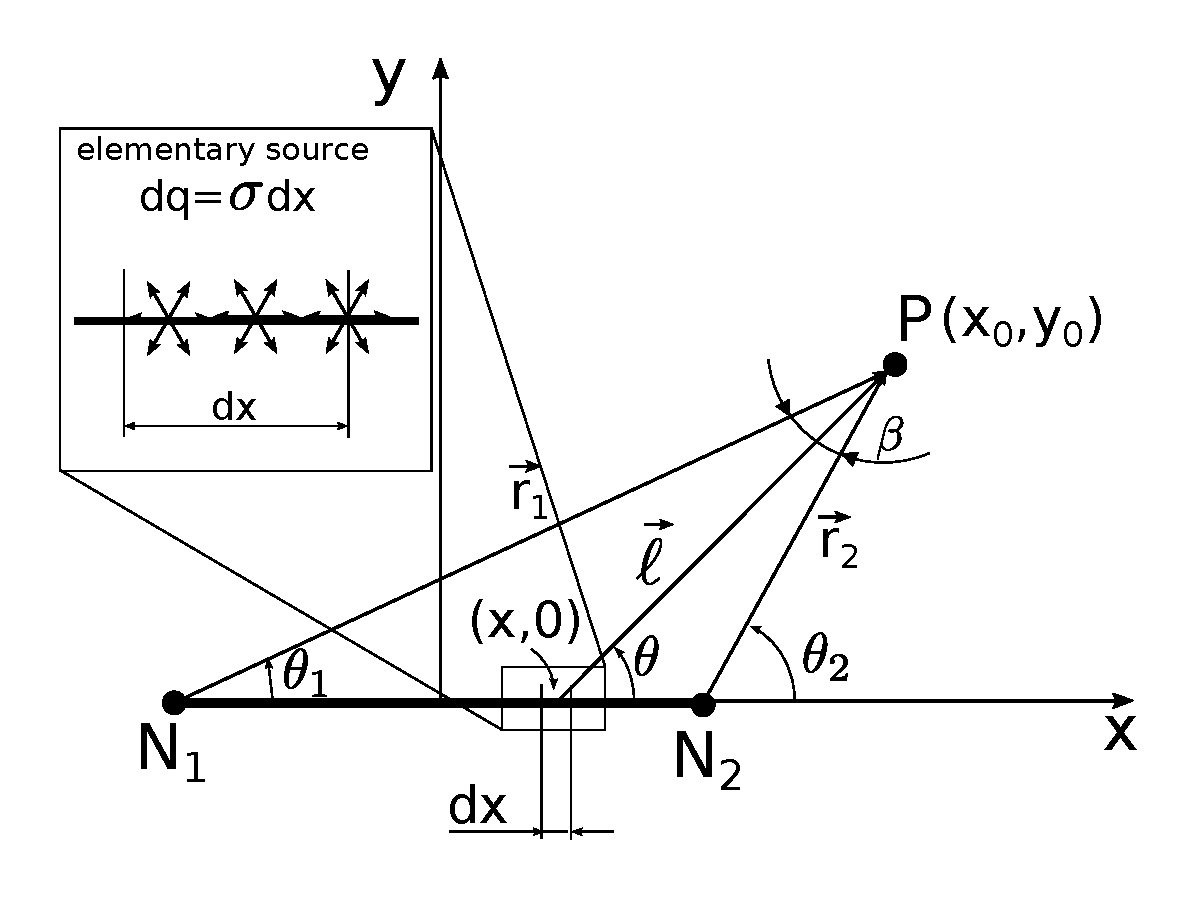
\includegraphics[width=0.50\textwidth]{./fig/lineSource}
\caption{Rappresentazione di una sorgente puntiforme e della sorgente distribuita sul segmento $\bm{N}_1 \bm{N}_2$: definizione della ``densità lineare di sorgente'' $\sigma$ e  delle quantità geometriche.}\label{fig:lineSource}
\end{figure}
\end{center}

\noindent
Facendo riferimento alla figura \ref{fig:lineSource}, i punti appartenenti al segmento hanno coordinate $(x,0)$, con $x \in (x_{N_1},x_{N_2})$. 
%
Il contributo elementare di velocità indotta nel punto $\bm{P}$ dal segmento di lunghezza infinitesima $dx$ vale
\begin{equation}
 d\bm{u} = \dfrac{\sigma dx}{2\pi \ell} \bm{\hat{\ell}} = \dfrac{\sigma dx}{2\pi \ell^2} \bm{\ell} \ ,
\end{equation}
avendo indicato con $\bm{\ell} = (x_0 - x) \, \bm{\hat{x}} + y_0 \, \bm{\hat{y}}$ il vettore di lunghezza $\ell$ che congiunge il generico punto sul segmento $\bm{N}_1 \bm{N}_2$ con il punto $\bm{P}$ e con $\bm{\hat{\ell}} = \bm{\ell} / \ell$ il versore che ne identifica la direzione.
%
Per risolvere il problema risulta comodo esprimere la coordinata $x$ in funzione dell'angolo $\theta$ formato dal vettore $\bm{\ell}$ con l'asse $x$ e usare l'angolo $\theta$ come coordinata indipendente per parametrizzare i punti del segmento. Si può scrivere
\begin{equation}
 \bm{\ell} = \ell \cos \theta \bm{\hat{x}} + \ell \sin \theta \bm{\hat{y}} = 
 (x_0 - x) \bm{\hat{x}} + y_0 \bm{\hat{x}} \ ,
\end{equation}
per ricavare il legame tra $x$ e $\theta$,
\begin{equation}
 \ell \cos \theta = x_0 - x \qquad , \qquad \ell \sin \theta = y_0 \qquad \rightarrow \qquad x-x_0 = y_0 \dfrac{\cos \theta}{\sin \theta} \ ,
\end{equation}
e l'espressione che lega i differenziali $dx$ e $d\theta$,
\begin{equation}
 dx = \dfrac{y_0}{\sin^2 \theta} d \theta \ .
\end{equation}
Se la sorgente ha densità uniforme unitaria, allora $\sigma = 1$ e si può scrivere
%
\begin{equation}
\begin{aligned}
 d\bm{u} & = \dfrac{1}{2\pi} \dfrac{1}{\ell^2} \ \bm{\ell}\  dx = \\
 & = \dfrac{1}{2\pi} \dfrac{\sin^2 \theta}{y_0^2} \left[ y_0 \dfrac{\cos \theta}{ \sin \theta} \bm{\hat{x}} + y_0 \bm{\hat{y}} \right] \ \dfrac{y_0}{\sin^2 \theta} d\theta = \\
 & = \dfrac{1}{2\pi} \left[ \dfrac{\cos \theta}{\sin \theta} \bm{\hat{x}} + \bm{\hat{y}} \right] d \theta 
\end{aligned}
\end{equation}
%
Per ottenere il contributo integrale di tutta la sorgente lineare, è necessario svolgere l'integrale del contributo elementare su tutto il segmento
\begin{equation}
\begin{aligned}
 \bm{u} & = \int_{\bm{N}_1}^{\bm{N}_2} d\bm{u} = \\
 & = \dfrac{1}{2\pi} \int_{\theta_1}^{\theta_2} \left[ \dfrac{\cos \theta}{\sin \theta} \bm{\hat{x}} + \bm{\hat{y}} \right] d \theta  = \\
 & = \dfrac{1}{2\pi} \left[ \ln \dfrac{\sin \theta_2}{\sin \theta_1} \bm{\hat{x}} + (\theta_2 - \theta_1 ) \bm{\hat{y}} \right] = \\
 & = - \dfrac{1}{2\pi} \ln \dfrac{|\bm{r}_2|}{|\bm{r}_1|} \bm{\hat{x}} 
 + \dfrac{1}{2\pi} \beta \bm{\hat{y}} \ .
\end{aligned}
\end{equation}
L'ultima espressione è stata ricavata utilizzando il legame $\theta_2 = \theta_1 + \beta$ tra angoli interni ed esterni di un triangolo ed elaborando il termine del logaritmo come
\begin{equation}
 \ln \dfrac{\sin \theta_2}{\sin \theta_1} =
 \ln \dfrac{\sin \theta_2 / y_0}{\sin \theta_1 / y_0} =
 \ln \dfrac{1 / |\bm{r}_2|}{ 1 / |\bm{r}_1|} =
 \ln \dfrac{ |\bm{r}_1| }{ |\bm{r}_2| } =
 - \ln \dfrac{ |\bm{r}_2| }{ |\bm{r}_1| } \ . 
\end{equation}

\vspace{3.0cm}
\noindent
